\section{Visual Regression Testing Infrastructure}

\subsection{Introduction}

Modern web applications evolve continuously, and frequent modifications to the \acs{UI} can unintentionally introduce visual defects. Traditional software testing approaches, such as unit and integration testing, mainly verify application behavior, business logic, and component structure. However, they are not sufficient to detect presentation-level regressions affecting layout, typography, colors, images, or component positioning.

To address this limitation, a \acs{VRT} infrastructure was introduced using \textbf{Reg-Suit}. This system automatically captures application screenshots, compares them against approved reference images, detects visual differences, and generates reports that facilitate review during the \acs{CI} workflow.

The implemented solution targets initially the \texttt{next-common} project and covers two major application areas:

\begin{itemize}
    \item Storybook component stories visual testing.
    \item \acf{E2E} page visual testing.
\end{itemize}


\subsection{Visual Regression Testing}

\subsubsection{Definition}

Visual Regression Testing is a testing technique that detects unintended changes in the rendered appearance of a \ac{UI} by comparing screenshots generated from different application versions.

Unlike traditional automated tests that validate HTML structure, component properties, or application behavior, \ac{VRT} operates at the presentation layer. Any modification affecting the visual output, such as spacing, typography, colors, icons, images, or element positioning, can be detected through a pixel-based comparison.

\subsubsection{Testing Workflow}

The visual regression workflow consists of three main phases:

\begin{enumerate}
    \item \textbf{Snapshot generation:} screenshots are captured from the current application version.
    
    \item \textbf{Baseline comparison:} the generated screenshots are compared against reference snapshots stored from a previous validated version.
    
    \item \textbf{Difference analysis:} a pixel-level comparison algorithm identifies visual changes according to a predefined threshold and generates a visual regression report.
\end{enumerate}

\subsubsection{Reg-Suit}

\textbf{Reg-Suit} is the open-source tool selected to implement the comparison and reporting layer of the \ac{VRT} infrastructure. It is built around a plugin architecture that separates three concerns: identifying which snapshots to compare (key generation), performing the actual pixel comparison, and publishing the resulting artifacts to a storage backend. In the workflow of this project, Reg-Suit is responsible for:

\begin{itemize}
    \item Retrieving the actual (current) and expected (baseline) screenshot sets.
    \item Performing an automated pixel-based comparison between the two sets.
    \item Generating an interactive HTML report, backed by a JSON result file, that highlights every detected difference.
    \item Publishing the screenshots and the report to a cloud storage bucket so that they can be reviewed outside the \ac{CI} runner.
\end{itemize}

Reg-Suit is maintained as an open-source project and is available on its official GitHub repository\footnote{Reg-Suit official repository: \url{https://github.com/reg-viz/reg-suit}}, which also hosts the plugin ecosystem (key generation, publishing, and notification plugins) used to adapt the tool to different \ac{CI} and storage environments \cite{regsuit_repo}.

\subsection{Storybook Stories Screenshot Preparation}

As introduced in the section \ref{sec:storybook-upgrade}, Storybook is used throughout the \texttt{next-common} project as the primary environment for developing and testing \ac{UI} components in isolation. Because every component already has one or more stories describing its states, Storybook naturally became the entry point for component-level \ac{VRT}: instead of writing dedicated visual test cases, existing stories are reused directly as the source of truth for screenshot generation.

\subsubsection{Building Storybook}

Before any screenshot can be captured, the Storybook application is built into a static bundle. Building it upfront, rather than capturing screenshots against a live development server, provides a lightweight and quickly accessible environment: the static build can be served directly to the screenshot workers without incurring the overhead of Storybook's development server (hot module reloading, on-the-fly compilation, etc.), which significantly improves the stability and speed of the capture phase.

This step is not a minor implementation detail. The project currently contains more than \textbf{1,000 stories}. Once the supported dark/light themes and the supported languages are taken into account, the number of individual screenshots that may need to be generated for a full run can reach approximately \textbf{12,000}. At this scale, both the time required to generate screenshots and the storage cost of keeping them in the cloud become first-class engineering concerns, which directly motivated the parallelization strategy described below.

\subsubsection{Automated Screenshot Generation}

A dedicated script automates the generation of screenshots for every Storybook story, so that the process requires no manual intervention and can run unattended in \ac{CI}.

\paragraph{Algorithm}

\begin{enumerate}
    \item Create a pool of worker processes: \textbf{8 workers} when running locally, and \textbf{16 workers} when running in \ac{CI}, where more compute is available.
    \item Build the Storybook application into a static bundle.
    \item Read the generated \texttt{index.json} file, which lists every available story together with its identifier and metadata.
    \item Distribute the list of stories evenly across the pool of workers.
    \item Execute the workers concurrently, each one driving its own browser instance.
    \item For each assigned story, navigate to it and capture a screenshot once the component has finished rendering.
    \item Store the resulting screenshot in the designated snapshots directory, following a naming convention derived from the story identifier, theme, and language.
\end{enumerate}

By distributing the capture work across multiple concurrent workers rather than generating screenshots sequentially, the total time required to produce the complete set of Storybook screenshots is reduced by roughly the same factor as the number of workers, which is essential given the volume of stories described above.

\subsubsection{Storybook-Related Commands}

To simplify the workflow for developers and for the \ac{CI} pipeline, dedicated commands were added to the project:

\begin{lstlisting}[language=bash]
# Build the Storybook static bundle
pnpm book:build

# Generate screenshots for every story
pnpm book:screenshots
\end{lstlisting}

These commands abstract away the details of the build and capture algorithm described above, so that both local developers and \ac{CI} jobs can trigger a full Storybook screenshot generation with a single invocation.

The output of the \texttt{book:screenshots} command is a set of PNG files, one for each story, stored in the \texttt{\_\_storybook\_screenshots\_\_/} directory. This directory is then used as the input for the Reg-Suit comparison phase, which retrieves the corresponding baseline screenshots and produces a visual regression report.

\subsection{End-to-End Tests}

\subsubsection{Definition}

End-to-end testing is a testing method that validates a complete software workflow by exercising the application the way a real user would, across every layer of the stack, from the user interface down through its integrations, rather than testing an isolated unit or component in artificial conditions \cite{istqb_e2e}. According to the \ac{ISTQB} glossary, end-to-end testing consists of validating business processes from start to finish under production-like circumstances \cite{istqb_e2e}, an approach that is also discussed at length as part of the system and acceptance testing levels in the standard \ac{ISTQB} testing literature \cite{black_foundations}.


In the context of this project, \ac{E2E} tests are used not only to validate functional behavior but also as the trigger points from which visual screenshots are captured, since they reproduce realistic, fully rendered application states.

\subsubsection{E2E Test Architecture}
 
To make \ac{E2E} tests deterministic and independent from any external service, a fully controlled test environment was built around five building blocks: a mock server, mocked services, mocked data, reusable fixtures, and a dedicated mock application exercised by the Playwright test suite itself.
 
\paragraph{Mock Server} The \texttt{mocks-server} package is used to serve mocked \ac{API} responses in place of the real backend. It intercepts outgoing requests from the application under test and returns predefined responses and status codes, which removes any dependency on external services, network availability, or backend state during test execution.
 
\paragraph{Mocked Services} A mocked service reproduces the expected behavior of a real service, returning predefined responses when invoked so that development and testing happen in a controlled, predictable environment, without depending on the real service or its own external dependencies.
 
\textbf{Important:} A \textbf{mocked service} is the fake behavior itself but the \textbf{mock server} is the infrastructure that exposes one or more mocked services as network endpoints.

A suitable example illustrating this distinction is when a method retrieves data from a specific URL that cannot be handled by the mock server. In such a case, the mocked service can be used to simulate the expected behavior by returning a predefined response instead of executing the original method against the real service.
 
\paragraph{Mocked Data} The responses served by the mock server are stored as plain JSON fixture files within the codebase. Keeping them as versioned files, rather than generating them dynamically, guarantees that the exact same data set is used across every test run, which is a prerequisite for producing stable, comparable screenshots.
 
\paragraph{Fixtures} Playwright fixtures are used to configure reusable test environments, data, and setup procedures. They encapsulate common preconditions, such as navigating to a given page with a given mocked state, so that individual test files stay focused on the scenario being validated instead of repeating boilerplate setup logic.
 
\paragraph{Mock Application} A dedicated Next.js application was built specifically to host the pages required for \ac{E2E} testing, including:
 
\begin{itemize}
    \item \texttt{/product}
    \item \texttt{/merchant-center}
\end{itemize}
 
This mock application uses the mocked services and consumes the mock server with the mocked data described above. By simply updating the \texttt{API\_ENDPOINT} environment variable to point to the mock server's URL, each rendered page reproduces a fixed and predictable application scenario without relying on any external or production services.
 
\paragraph{Playwright Tests} Approximately \textbf{40 \ac{E2E} tests} were implemented using Playwright against the mock application. These tests exercise the main user scenarios and validate that the expected content, layout, and interactive elements are present, providing the functional coverage on top of which visual screenshots are captured.

\subsubsection{Screenshot Generation}

Playwright is configured to capture a screenshot at the relevant point of each \ac{E2E} test. The screenshot configuration defines parameters such as the viewport size and full-page versus element-level capture. Rendering is also constrained to a consistent browser (Chromium) engine and viewport across local and \ac{CI} runs, so that differences in the underlying rendering environment do not introduce false positives.

\subsubsection{Project Commands}

The following commands were added to the \texttt{package.json} of the mocked application to simplify the \ac{E2E} workflow:

\begin{lstlisting}[language=bash]
# Start the mock server
pnpm mocks:start

# Start the mocked Next.js application
pnpm start

# Execute the Playwright E2E test suite
pnpm test:e2e

# Generate the required screenshots
pnpm test:visual:e2e
\end{lstlisting}

\subsection{Reg-Suit Configuration}

As previously mentioned, Reg-Suit is the testing framework used to perform visual comparisons and generate the corresponding report.

\subsubsection{Dependencies and Plugins}

Reg-Suit is installed together with the plugins required to identify snapshots and to publish comparison artifacts. The relevant packages are declared as \texttt{devDependencies}:

\begin{lstlisting}[language=json]
{
  "devDependencies": {
    "reg-suit": "^0.16.2",
    "reg-keygen-git-hash-plugin": "^0.16.2",
    "reg-simple-keygen-plugin": "^1.0.0",
    "reg-publish-gcs-plugin": "^0.6.0"
  }
}
\end{lstlisting}

\begin{itemize}
    \item \textbf{\texttt{reg-suit}}: the main plugin, responsible for orchestrating the comparison lifecycle (fetching snapshots, comparing them, and generating the report).
    \item \textbf{\texttt{reg-keygen-git-hash-plugin}}: a Git-based key generation plugin that derives the actual and expected snapshot keys from the local Git history. It is primarily used for local development, where the actual snapshot corresponds to the latest commit on the current branch, while the expected snapshot corresponds to the base commit from which the branch was created.
    \item \textbf{\texttt{reg-simple-keygen-plugin}}: a simple key generation plugin that accepts the actual and expected keys explicitly as configuration values or environment variables used in both local and \ac{CI} contexts.
    \item \textbf{\texttt{reg-publish-gcs-plugin}}: publishes the comparison artifacts (screenshots and report) to a Google Cloud Storage bucket.
\end{itemize}

\subsubsection{Reg-Suit Configuration File}

Reg-Suit is configured through a JSON configuration file, one for the Storybook stories and one for the \ac{E2E} tests, so that both can run and coexist independently. An example configuration is shown below:

\begin{lstlisting}[language=json]
{
  "core": {
    "workingDir": ".reg-e2e", // or ".reg-sb" for Storybook
    "actualDir": "__e2e_tests_screenshots__/", // or "__storybook_screenshots__/" for Storybook
    "thresholdRate": 0.0001
  },
  "plugins": {
    "reg-simple-keygen-plugin": {
      "actualKey": "<ACTUAL_SHA>",
      "expectedKey": "<EXPECTED_SHA>"
    },
    "reg-publish-gcs-plugin": {
      "bucketName": "<BUCKET_NAME>",
      "pathPrefix": "<FOLDER_PATH>"
    }
  }
}
\end{lstlisting}

\paragraph{Working Directories}

The \texttt{workingDir} parameter defines the temporary directory used by Reg-Suit during execution. Once execution completes, this directory holds the generated screenshots retrieved for comparison, the corresponding baseline screenshots, the pixel-level difference images, the JSON comparison result (\texttt{out.json}), and the HTML report itself (\texttt{index.html}).

Separate working directories, \texttt{.reg-sb} for Storybook and \texttt{.reg-e2e} for \ac{E2E}, are used so that both reports can be generated and stored independently without overwriting one another.

\paragraph{Threshold}

The \texttt{thresholdRate} parameter defines the maximum acceptable ratio of differing pixels between an actual screenshot and its baseline before the comparison is flagged as a regression. The configured value, \texttt{thresholdRate = 0.0001}, means that a screenshot is reported as failed once more than $0.01\%$ of its pixels differ from the baseline. This deliberately strict threshold favors sensitivity: it catches subtle visual regressions while the noise-reduction mechanisms described later in this section (disabled animations, mocked data, asset-loading waits) keep false positives to a minimum.

\paragraph{Git Plugin Key Generation}

For local development, the \texttt{reg-keygen-git-hash-plugin} is used so that developers do not need to manually provide commit hashes. The plugin inspects the local Git repository and automatically derives the actual key from the current working tree and the expected key from the last known baseline commit, which keeps the local workflow lightweight.

\paragraph{Simple Key Generation}

The \texttt{reg-simple-keygen-plugin} is used when the actual and expected snapshot keys must be specified explicitly rather than inferred from the local Git state. This applies to local runs where a specific baseline needs to be targeted and, more importantly, to \ac{CI} execution. In the latter case, the actual key corresponds to the merge-base commit \ac{SHA}, while the expected key corresponds to the target branch (typically \texttt{main} or \texttt{master}) commit \ac{SHA}, with both values either computed by the pipeline or provided through a workflow dispatch event.

\paragraph{Cloud Storage}

Two storage backends are used depending on the execution environment:

\begin{itemize}
    \item \textbf{Local development}: An S3-compatible object store is provided by \textbf{s3rver}. It persists objects under the \texttt{.s3-data/} directory and exposes an S3-compatible endpoint at \texttt{http://localhost:4568}. This eliminates the need for real cloud credentials during the development and debugging of the \ac{VRT} setup.

    \item \textbf{\ac{CI} execution}: Google Cloud Storage (\ac{GCS}) is used as the production storage backend. It provides persistent storage for snapshots and reports generated by the pipeline, allowing them to be reused across different pull request runs.
\end{itemize}

The storage is organized according to the following conventions:

\begin{itemize}
    \item \textbf{Bucket naming}: The repository name is used as the bucket name, allowing each \texttt{fo-app} to have its own dedicated storage bucket. For example, the \texttt{next-common} project uses the \texttt{gs://next-common} bucket.

    \item \textbf{pathPrefix}: Each bucket contains two objects (folders), \texttt{storybook} and \texttt{end\_2\_end}, which store the reports and snapshots associated with their respective testing surfaces. Each report is identified using the naming convention
    \[
        \texttt{<actual\_sha>-vs-<expected\_sha>}
    \]
    allowing multiple reports to coexist within the same bucket without overwriting one another.
\end{itemize}

\subsubsection{Project Commands}

The following commands were added to drive the Reg-Suit workflow:

\begin{lstlisting}[language=bash]
# Local execution (Storybook / E2E)
pnpm reg:run:sb:local
pnpm reg:run:e2e:local

# Remote execution against GCS (Storybook / E2E)
pnpm reg:run:sb:remote
pnpm reg:run:e2e:remote

# Open a generated report locally
pnpm reg:open:sb
pnpm reg:open:e2e
\end{lstlisting}

Each \texttt{reg:run:*} command wraps the standard \texttt{regsuit run} invocation: it takes the freshly generated screenshots, retrieves the corresponding baseline, runs the comparison, generates the HTML/JSON report, and publishes the resulting artifacts to the configured storage backend, all in a single step.

\subsection{Visual Regression Testing in CI}

\subsubsection{Objective}

The \ac{VRT} workflow is triggered automatically whenever a \ac{PR} is opened or updated. Its objective is to compare the screenshots produced from the base branch (Usually \textbf{\texttt{main}}) against the screenshots produced from the \textbf{mergeable version of the \ac{PR}}, so that reviewers can directly inspect the resulting report to identify visual regressions, instead of having to check out the branch locally and manually walk through every page or component. Beyond manual review, the structured, machine-readable comparison output (the \texttt{out.json} result) also opens the door to a further enhancement: automating part of the \ac{PR} review process using \ac{AI}, by feeding the detected differences to a model capable of triaging intentional design changes from genuine regressions.

\subsubsection{GitHub Actions}

The \ac{VRT} workflow is implemented as a GitHub Actions workflow, defined in \texttt{\allowbreak .github/workflows/reg-vis-suit.yml}. It is divided into four jobs to optimize the overall execution time, release runner resources as early as possible, and avoid regenerating screenshots that are already available from previous runs.

\textbf{Note:} GitHub Actions jobs run in parallel by default. However, a dependency between jobs must be declared explicitly using the \texttt{needs} keyword whenever one job depends on the output of another. This behavior is deliberately leveraged in the workflow design described in the following sections.

\subsubsection{CI Workflow}

\paragraph{Job 1 --- Retrieve and Validate Commits}

The first job serves as the initialization and validation stage of the visual regression testing workflow. It determines the commit SHAs involved in the comparison, checks the availability of their corresponding snapshots in \ac{GCS}, and exposes the resulting information to the subsequent jobs. It consists of the following steps:

\begin{enumerate}
    \item \textbf{Determine the actual commit SHA}: Retrieve the commit SHA corresponding to the mergeable version of the pull request. When the workflow is triggered by a workflow dispatch event, the SHA is instead obtained from the provided workflow inputs.

    \item \textbf{Determine the expected commit SHA}: Retrieve the commit SHA corresponding to the target branch, typically \texttt{main}. When the workflow is triggered by a workflow dispatch event, the SHA is instead obtained from the provided workflow inputs.

    \item \textbf{Check the actual snapshots}: Verify whether the screenshots associated with the actual commit SHA are already available in \ac{GCS}.

    \item \textbf{Check the expected snapshots}: Verify whether the screenshots associated with the expected commit SHA are already available in \ac{GCS}.

    \item \textbf{Expose job outputs}: Make the determined commit SHAs and snapshot availability information available as job outputs. These outputs are consumed by subsequent jobs to determine whether snapshot generation is required.
\end{enumerate}

\paragraph{Job 2 --- Generate Actual Snapshots}

This job generates and publishes to \ac{GCS} the screenshots corresponding to the mergeable version of the pull request. It is conditionally executed based on the snapshot availability determined by \textbf{Job 1}. If the corresponding snapshots already exist in \ac{GCS}, the job is skipped, avoiding redundant screenshot generation and reducing the consumption of CI runner resources.

\paragraph{Job 3 --- Generate Expected Snapshots}

This job generates and publishes to \ac{GCS} the baseline screenshots corresponding to the target branch commit, typically \texttt{main}. It is independent of \textbf{Job 2} and therefore runs in parallel with it, reducing the overall execution time of the workflow. Similarly, the job is skipped when \textbf{Job 1} determines that the corresponding snapshots are already available in \ac{GCS}. This is particularly beneficial when multiple pull requests share the same target branch commit, as the same baseline snapshots can be reused across workflow runs.

Since Jobs 2 and 3 perform the same sequence of operations but operate on different commits and snapshot keys, their common logic is encapsulated in a reusable local action located at \path{.github/actions/generate-screenshots}. Both jobs invoke this action with their respective inputs, eliminating duplicated workflow logic and ensuring that the screenshot generation process remains consistent across both execution paths.

The reusable action performs the following steps:

\begin{enumerate}
    \item \textbf{Checkout the repository}: Checkout the repository at the commit specified by the provided input.

    \item \textbf{Set up the environment}: Install and configure the required versions of Node.js and \texttt{pnpm}.

    \item \textbf{Install dependencies}: Install the project dependencies required to build the application and generate the screenshots.

    \item \textbf{Authenticate with Google Cloud}: Authenticate with Google Cloud using credentials securely provided through workflow secrets.

    \item \textbf{Generate Storybook screenshots}: Build and serve the Storybook bundle, then capture screenshots of the configured stories.

    \item \textbf{Generate the Reg-Suit configuration for Storybook}: Dynamically generate the Reg-Suit configuration for the Storybook snapshots using the appropriate snapshot key and storage configuration. A dedicated script is used to automate this configuration.

    \item \textbf{Run the visual comparison for Storybook}: Execute Reg-Suit to process the generated Storybook snapshots and publish them to \ac{GCS}.

    \item \textbf{Generate E2E test screenshots}: Start the E2E mock server and mock application, then execute the end-to-end tests to capture the corresponding screenshots.

    \item \textbf{Generate the Reg-Suit configuration for E2E tests}: Dynamically generate the Reg-Suit configuration for the E2E snapshots using the appropriate snapshot key and storage configuration. The same configuration script used for Storybook is reused with parameters specific to the E2E testing surface.

    \item \textbf{Run the visual comparison for E2E tests}: Execute Reg-Suit to process the generated E2E snapshots and publish them to \ac{GCS}.
\end{enumerate}

\paragraph{Job 4 --- Compare and Publish Results}

The final job depends on both \textbf{Job 2} and \textbf{Job 3} and starts only after the required snapshot sets are available in \ac{GCS}. It retrieves the generated snapshots, performs the visual comparisons for both testing surfaces, and publishes the resulting reports and summaries.

It performs the following steps:

\begin{enumerate}
    \item \textbf{Checkout the repository}: Checkout the repository at the mergeable version of the pull request.

    \item \textbf{Set up the environment}

    \item \textbf{Install dependencies}

    \item \textbf{Authenticate with Google Cloud}

    \item \textbf{Download snapshots}: Download the actual and expected snapshot sets for both Storybook and E2E tests from \ac{GCS}. Each snapshot set is placed in its dedicated directory within the Reg-Suit working directory to keep the two testing surfaces isolated and prevent files from being overwritten.

    \item \textbf{Generate the Reg-Suit Storybook configuration}: Dynamically generate the Reg-Suit configuration required to compare the actual and expected Storybook snapshots.

    \item \textbf{Run the visual comparison for Storybook}: Execute Reg-Suit to compare the actual and expected Storybook snapshots and generate the corresponding visual regression report.

    \item \textbf{Generate the Reg-Suit E2E configuration}: Dynamically generate the Reg-Suit configuration required to compare the actual and expected E2E snapshots.

    \item \textbf{Run the visual comparison for E2E}: Execute Reg-Suit to compare the actual and expected E2E snapshots and generate the corresponding visual regression report.

    \item \textbf{Generate the comparison summary}: Parse the generated \texttt{out.json} files for both testing surfaces, extract the relevant comparison results, and build a human-readable summary in \acs{MD} format.

    \item \textbf{Publish the job summary}: Publish the generated summary as a GitHub Actions job summary, making the comparison results directly accessible from the workflow run.

    \item \textbf{Publish the PR comment}: If the workflow was triggered by a pull request, publish the generated summary as a comment on the corresponding PR. If a previous comment generated by the workflow already exists, update it instead of creating a new comment. This step is skipped when the workflow is triggered by a workflow dispatch event.
\end{enumerate}

The resulting pull request comment consolidates the results of both testing surfaces into a single, actionable report. It provides a link to the complete Storybook \ac{VRT} report, followed by a summary of the Storybook comparison results and a table containing the first ten detected visual differences. The comment then provides the corresponding link to the complete E2E \ac{VRT} report, together with a summary of the E2E comparison results and a table listing its first ten detected visual differences. This consolidated presentation allows developers to quickly assess the overall visual regression status of the pull request while retaining direct access to the complete reports for further investigation.

Figure~\ref{fig:regvis_workflow_jobs} illustrates the GitHub Actions workflow used to execute the Reg-Suit \ac{VRT} workflow. It shows the different jobs involved in the workflow and their execution dependencies.

\begin{figure}[H]
    \centering
    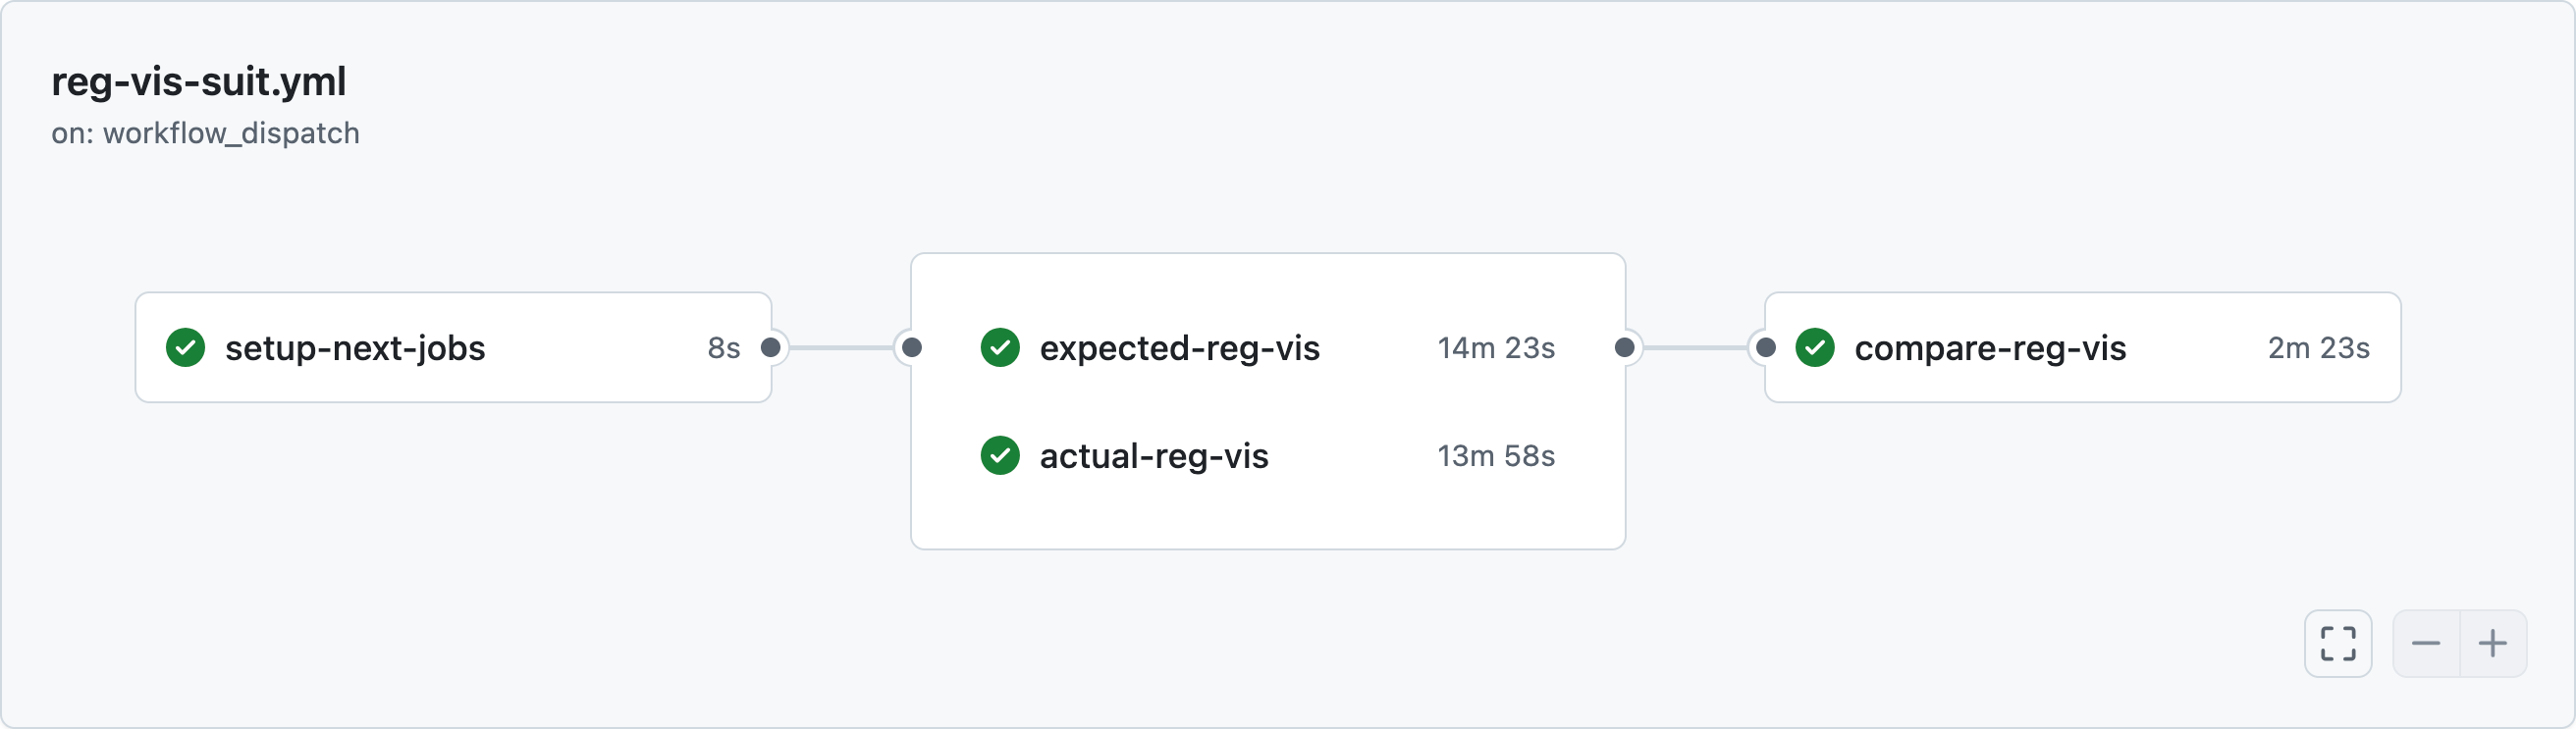
\includegraphics[width=.95\textwidth]{../assets/vis_reg_tests/regvis_workflow_jobs.png}
    \caption{GitHub Actions workflow for the Reg-Suit visual regression testing process.}
    \label{fig:regvis_workflow_jobs}
\end{figure}


\subsubsection{Use Case Example}

To illustrate the practical value of the workflow, consider a simple but easy-to-overlook \ac{UI} change: the destination URLs of two buttons in the application footer are accidentally swapped. The application still builds successfully, and the existing functional test suite continues to pass because no application logic is broken and both buttons still point to valid URLs. However, the rendered \ac{UI} no longer matches the approved baseline.

Because \ac{VRT} compares the rendered output against the corresponding baseline screenshots, the affected screenshots are detected as visual regressions. The generated pull request comment immediately highlights the affected pages and provides direct access to the comparison report. The reviewer can therefore inspect a side-by-side comparison of the previous and current versions, as well as a difference view highlighting the changed regions in red. This makes the regression immediately visible without requiring the reviewer to manually navigate through the application and test each footer link.

Figure~\ref{fig:footer_2up} shows the \textit{2-up} comparison view provided by the \ac{VRT} report. The view displays the baseline (\textit{Before}) screenshot alongside the screenshot generated from the current pull request (\textit{After}), allowing the reviewer to identify the visual differences between the two versions.

\begin{figure}[H]
    \centering
    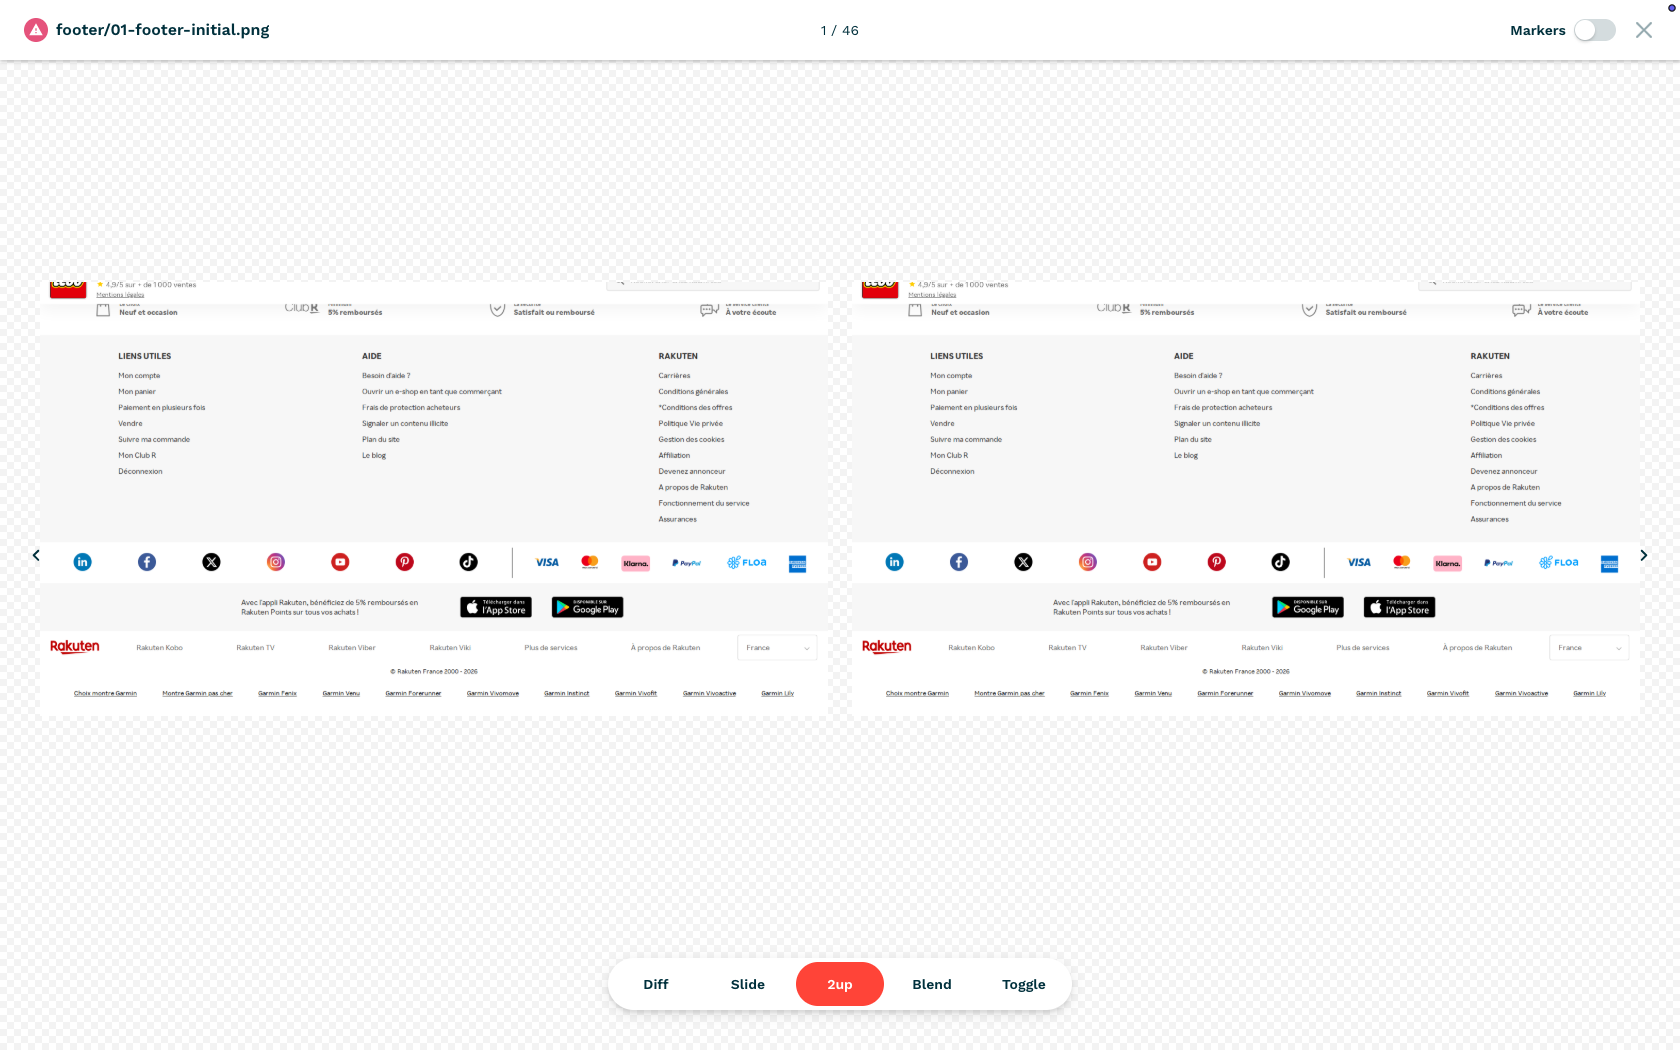
\includegraphics[width=.95\textwidth]{../assets/vis_reg_tests/footer_2up.png}
    \caption{2-up comparison showing the baseline and current versions of the application footer.}
    \label{fig:footer_2up}
\end{figure}

Figure~\ref{fig:footer_red_diff} shows the corresponding difference view of the same comparison. The detected visual changes are highlighted in red, making the affected regions immediately identifiable and allowing the reviewer to focus on the exact areas that differ from the baseline.

\begin{figure}[H]
    \centering
    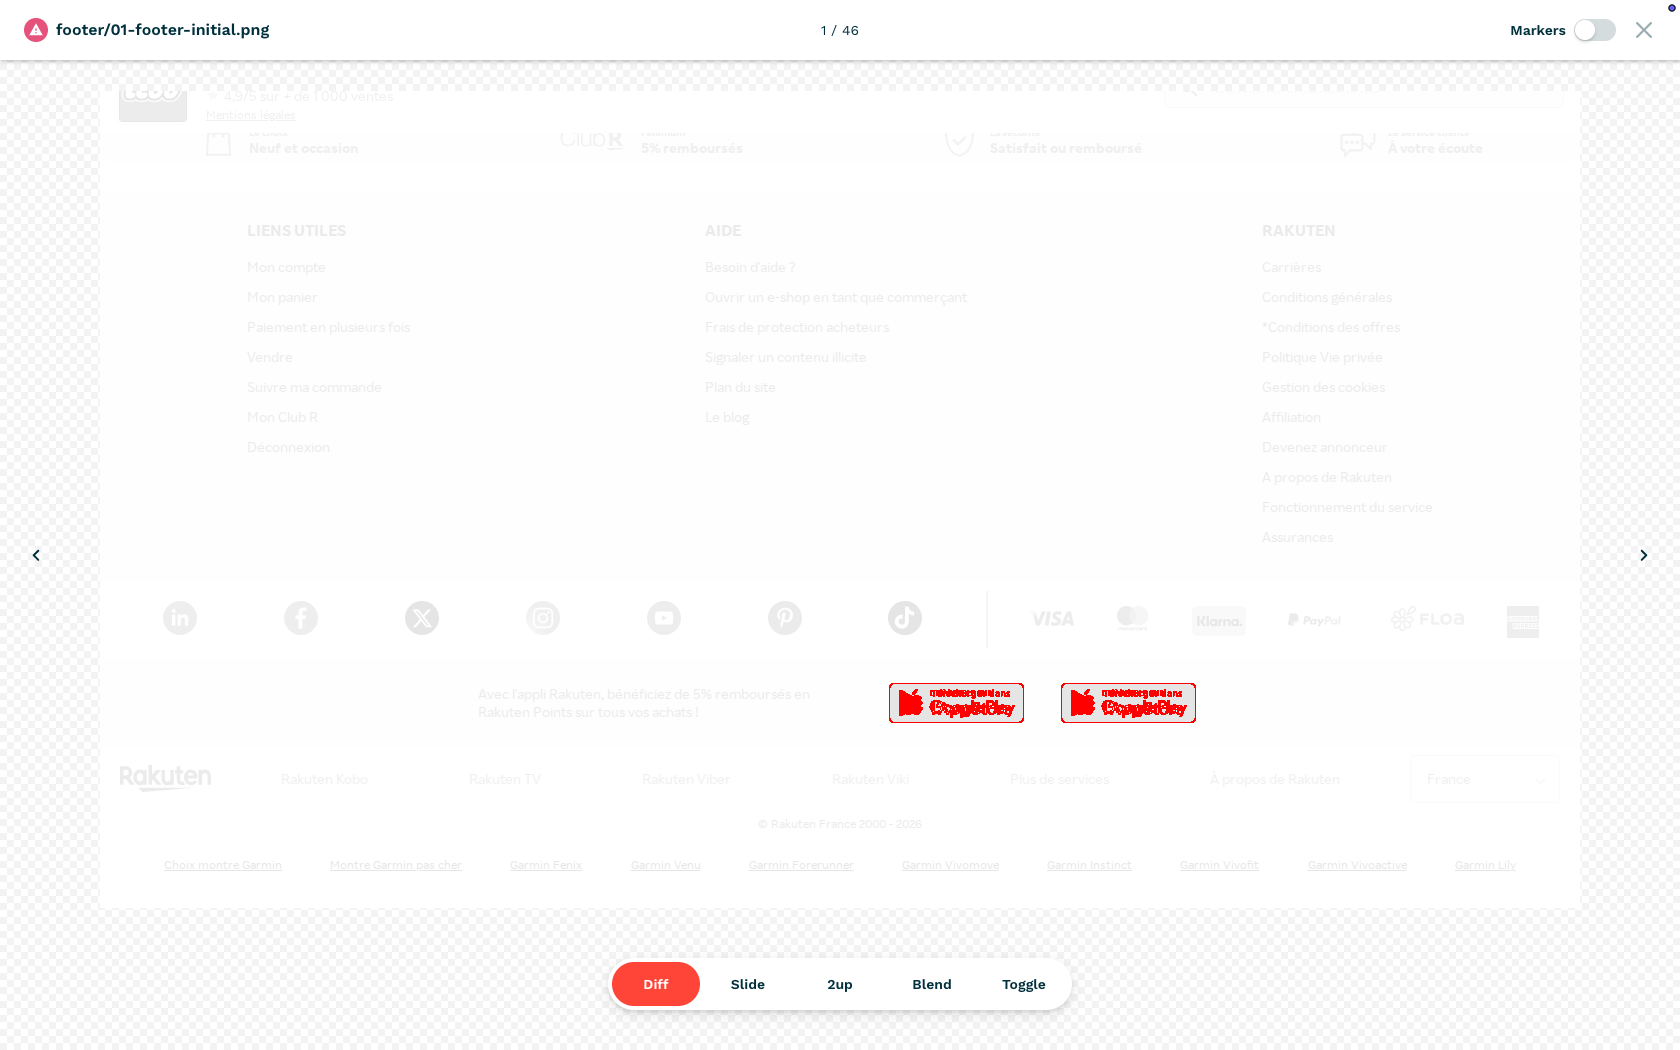
\includegraphics[width=.95\textwidth]{../assets/vis_reg_tests/footer_red_diff.png}
    \caption{Difference view highlighting the visual changes in the application footer.}
    \label{fig:footer_red_diff}
\end{figure}


\subsection{Conclusion and Future Improvement}

The \ac{VRT} infrastructure described in this section provides the \texttt{next-common} project with an automated mechanism for detecting unintended visual changes, at both the component level, through Storybook, and the application level, through \ac{E2E} pages. Its main benefits can be summarized as follows:

\begin{itemize}
    \item Automated visual validation, requiring no manual screenshot comparison.
    \item Coverage of both Storybook components and \ac{E2E} pages.
    \item Parallel screenshot generation, keeping execution time manageable despite the volume of stories and tests.
    \item Reusable snapshots stored in cloud storage, avoiding redundant regeneration across pull requests.
    \item Automatic comparison triggered on every pull request.
    \item Direct visibility of visual regressions through GitHub, via job summaries and pull request comments.
\end{itemize}

Despite these benefits, the current implementation has a known limitation: the Google Cloud Storage bucket used to store screenshots and reports is still \textbf{publicly accessible}. While this simplifies the retrieval of generated reports, both from the \ac{CI} pipeline and from a reviewer's browser, it introduces a security concern, since application screenshots and comparison artifacts should not necessarily be exposed publicly. This limitation directly motivates the next task in this project: implementing a secure \ac{HTTP} proxy in front of Google Cloud Storage, one that authenticates incoming requests and grants controlled access to private \ac{GCS} objects without exposing the storage bucket itself.

\clearpage
